\documentclass{resume}
\begin{document}
\fontfamily{ppl}\selectfont
\noindent
\begin{tabularx}{\linewidth}{@{}m{0.75\textwidth} m{0\textwidth}@{}}
{
    \large {Adwaid Sreeletha Anil} \newline
    \small{
    % \begin{align}
        Computer Science Student\newline
    % \end{align}
    \href{}{Address (Berliner Allee 199, Berlin, 13088} \textbf{·} \newline
        \clink{
            \href{https://adwaaaiith.github.io/Portfolio/}{Portfolio} \textbf{·}
            \href{mailto:adwaithh9383@gmail.com}{adwaithh9383@gmail.com} \textbf{·}
            \href{tel:+4917623862783}{+49 176 2386 2783}
            \textbf{·}
             \href{https://github.com/adwaaaiith/}{GitHub}\newline
             \href{https://www.linkedin.com/in/adwaid-sreeletha-anil-b49472403/}{LinkedIn}
             \textbf{·} 
             \newline
    }
}
}
& 
{
    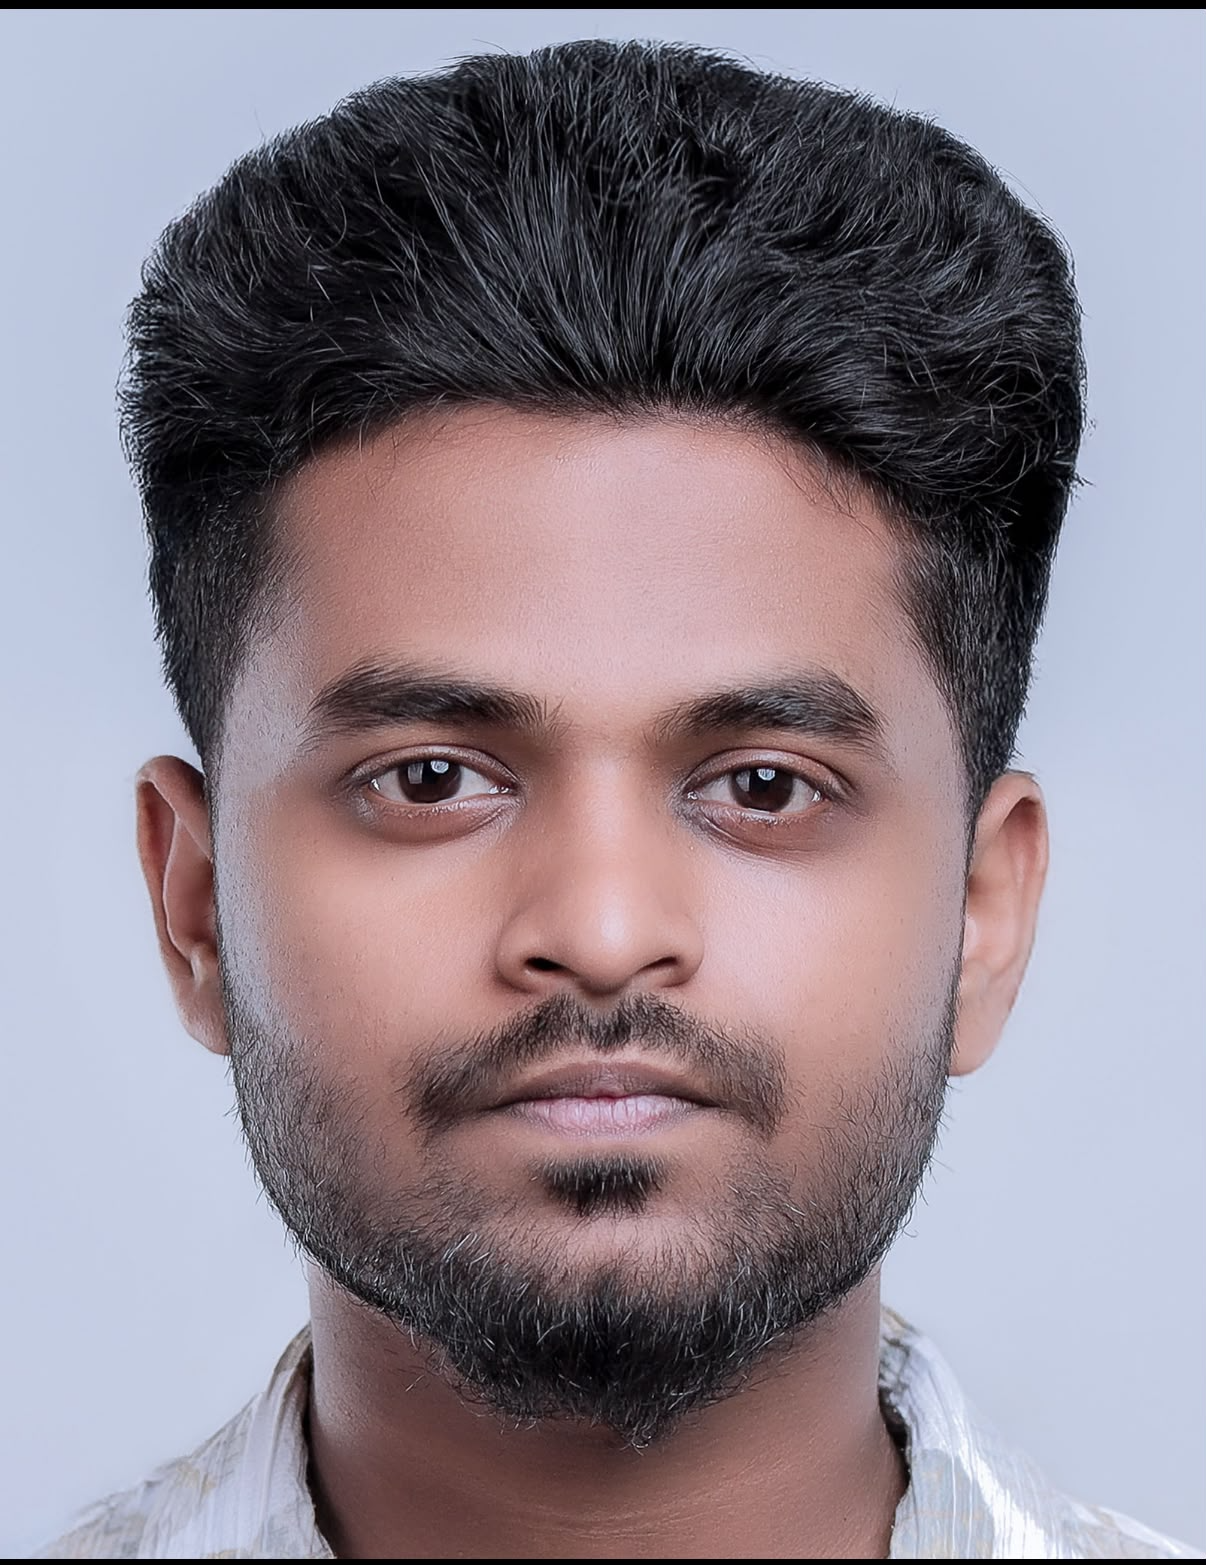
\includegraphics[width=4cm]{image.png}
}
\end{tabularx}
\csection{Summary}{\small
    \begin{itemize}
        \item \footnotesize Computer Science student at GISMA University of Applied Sciences with a strong interest in technology, programming, and web development. Currently building foundational skills in HTML, CSS, JavaScript, Linux, GitHub, and LaTeX through academic coursework and personal projects. Eager to learn, grow, and gain practical experience while developing a strong foundation in software development and computer science.
    \end{itemize}
}
\csection{EDUCATION}{\small
    \begin{itemize}
        % item 1 %
        \item \textbf{BSc Computer Science}\hspace{22em}(2026-2029)\newline{GISMA University of Applied Sciences,Berlin, Germany}\newline{Current Student}
        \item \textbf{Higher Secondary Education (Bio-Maths)}\hspace{12em}(2022--2024)
\newline{Kerala State Board, India}
        
    \end{itemize}
}
 
\csection{SKILLS}{\small
    \begin{itemize}
        \item \textbf{Technical Skills} \newline
        {\footnotesize HTML, CSS, Basic Javascript, Python (Beginner), Git, Github, Linux, LaTeX, Touch Typing  }{}{}
     
    \end{itemize}
}

\section{PROJECTS}{\small}
\begin{itemize}

\item \textbf{Personal Portfolio Website}
{\footnotesize

Built a responsive personal portfolio website using HTML, CSS and JavaScript.
Showcases my profile, technical skills, projects and contact information. Hosted using GitHub Pages.

\href{https://adwaaaiith.github.io/Portfolio/}{Live Demo} | \textbf{-}
\href{https://github.com/adwaaaiith/Portfolio}{GitHub}
}

\vspace{0.4cm}

\item \textbf{Scientific Calculator}
{\footnotesize

Developed a command-line scientific calculator using Python.
Implemented 15 mathematical operations including addition, subtraction, multiplication, division, power, square root, trigonometric functions, logarithms, factorial, percentage, and rounding.
Used loops, conditional statements, user input, and the Python \texttt{math} module to create an interactive calculator.

\href{https://github.com/adwaaaiith/Portfolio/blob/main/calculator.py}{GitHub}
}

\end{itemize}
    
\csection{EXPERIENCE}{\small
    \begin{itemize}
         \item \textbf{Warehouse Associate, DHL} \hspace{13em} Sep 2025 – Dec 2025
\newline Ludwigsfelde, Germany
    \end{itemize}
}
    
\csection{Global Certifications}{\small
    \begin{itemize}
        \item \textbf{German Language Certificate (A2)}
{\hspace{18em} 2024}{}
    \end{itemize}

}
        
\csection{Languages}{\small
\begin{itemize}
\item English (Fluent)
\item German (A2)
\item Malayalam (Native)
\end{itemize}

}



\end{document}